\documentclass[main.tex]{subfiles}
\begin{document}

\title{
    \textbf{Algorytmy ewolucyjne i metaheurystyki}\\
    \begin{large}
        Sprawozdanie 2
    \end{large}
}

\author{
    Górka Bartosz\\
  \texttt{127228}
  \and
  Zimniak Kajetan\\
  \texttt{127229}
}

\date{}

\maketitle

\section{Opis etapu projektu}
Celem kolejnego etapu projektu było wykorzystanie przygotowanego podczas ćwiczenia 1 środowiska testowego. W projekcie należało wykorzystać naiwny algorytm przydziału punktów do grup oraz algorytm losowy, które stanowiły podstawę tworzenia rozwiązania startowego dla algorytmów lokalnego przeszukiwania przygotowanych podczas tego etapu projektu.

Jako naiwny algorytm wykorzystano algorytm przydziału punktu do grupy (bez żalu), natomiast algorytm losowy został oparty o całkowicie losowy przydział każdego punktu do jednej z 20 grup.

W ramach projektu przygotowano dwa algorytmy przeszukiwania lokalnego. Pierwszym z nich jest algorytm \textit{Greedy Local Search}, natomiast drugim \textit{Steepest Local Search}.

Podobnie jak w poprzednim etapie, funkcja celu została zdefiniowana jako \textit{minimalizacja średniej odległości wszystkich par obiektów umieszczonych w ramach tej samej grupy}.

W rozdziale \ref{section:pseudokody} zaprezentowano pseudokody przygotowanych algorytmów, natomiast w rozdziale\leavevmode\nobreak\ \ref{section:wyniki} wyniki działania algorytmów dla 100 iteracji. Ostatni rozdział dotyczy wizualizacji najlepszych uzyskanych rozwiązań.

\section{Pseudokody algorytmów przeszukiwania lokalnego}
\label{section:pseudokody}
\subsection{Generowanie listy ruchów}
W algorytmach Greedy oraz Steepest Local Search wykorzystano metodę tworzącą listę możliwych ruchów dla aktualnego przydziału punktów do grup. Aby ułatwić zrozumienie algorytmów, wydzielono ją z pseudokodów i zaprezentowano osobno:

\begin{verbatim}
Zainicjalizuj listę ruchów jako pustą listę
Dla każdego punktu p z listy możliwych punktów {
    Dla każdej grupy g z listy grup {
        Jeżeli punkt p nie należy do grupy g {
            Do listy możliwych ruchów dodaj potencjalne przesunięcie punktu p
                z obecnej grupy do grupy g
        }
    }
}
Jako wynik metody zwróć listę ruchów
\end{verbatim}

\subsection{Greedy Local Search}
\begin{verbatim}
Wykonuj dopóki przydział punktów do grup ulega zmianie {
    Przygotuj listę możliwych ruchów dla obecnego sąsiedztwa
    Dokonaj losowego posortowania listy ruchów

    Dla każdego ruchu r z listy możliwych ruchów {
        Oblicz deltę zmiany funkcji celu dla ruchu r
        Jeżeli delta poprawia wartość funkcji celu {
            Oznacz że dokonano zmiany przydziału punktów (kolejna iteracja możliwa)
            Zaaplikuj ruch r
            Dokonaj aktualizacji aktualnej wartości funkcji celu
            Przerwij pętlę sprawdzania ruchów
        }
    }
}
\end{verbatim}

\subsection{Steepest Local Search}
\begin{verbatim}
Wykonuj dopóki przydział punktów do grup ulega zmianie {
    Przygotuj listę możliwych ruchów dla obecnego sąsiedztwa

    Dla każdego ruchu r z listy możliwych ruchów {
        Oblicz deltę zmiany funkcji celu dla ruchu r
        Jeżeli delta poprawia wartość funkcji celu {
            Zapamiętaj ruch jako dotychczas najlepszy
            Dokonaj aktualizacji aktualnej wartości funkcji celu
        }
    }

    Jeżeli dokonano zapamiętania ruchu (zmieniono funkcję celu) {
        Zaaplikuj najlepszy ruch (najbardziej poprawiajacy funkcję celu)
        Oznacz że dokonano zmiany przydziału punktów (aby wykonać kolejną iterację)
    }
}
\end{verbatim}

\section{Wyniki eksperymentów obliczeniowych}
\label{section:wyniki}
W tabeli \ref{table:wyniki} zaprezentowano wyniki eksperymentów obliczeniowych. Dokonano $100$ powtórzeń obliczeń. Za każdym razem algorytmy zostały uruchomione dla dwóch rozwiązań startowych. Pierwszy z nich to wynik działania algorytmu naiwnego przygotowanego w poprzednim ćwiczeniu, a drugi to przydział przygotowany przez algorytm losowego przydziału punktów do grup.
\begin{table}[H]
\centering
\caption{Wyniki eksperymentów obliczeniowych dla 100 iteracji}
\label{table:wyniki}
\resizebox{\textwidth}{!}{%
\begin{tabular}{|c|r|r|r|r|}
\hline
\textbf{Cecha} &                                                        \multicolumn{1}{c|}{\textbf{Naive Greedy LS}} & \multicolumn{1}{c|}{\textbf{Random Greedy LS}} & \multicolumn{1}{c|}{\textbf{Naive Steepest LS}} & \multicolumn{1}{c|}{\textbf{Random Steepest LS}} \\ \hline
\textbf{\begin{tabular}[c]{@{}c@{}}Wartość minimalna\\funkcji celu\end{tabular}}
&   26.39
&   26.37
&   26.39
&   26.39                                                 \\ \hline
\textbf{\begin{tabular}[c]{@{}c@{}}Wartość maksymalna\\funkcji celu\end{tabular}}
&   29.07
&   27.99
&   28.82
&   28.86                                                 \\ \hline
\textbf{\begin{tabular}[c]{@{}c@{}}Wartość średnia\\funkcji celu\end{tabular}}
&   27.00
&   26.95
&   27.27
&   27.12                                                  \\ \hline
\textbf{\begin{tabular}[c]{@{}c@{}}Wartość minimalna\\czasu obliczeń {[}sec{]}\end{tabular}}
&   0.11
&   0.34
&   0.83
&   4.50                                                  \\ \hline
\textbf{\begin{tabular}[c]{@{}c@{}}Wartość maksymalna\\czasu obliczeń {[}sec{]}\end{tabular}}
&   0.60
&   0.71
&   3.28
&   7.51                                                  \\ \hline
\textbf{\begin{tabular}[c]{@{}c@{}}Wartość średnia\\czasu obliczeń {[}sec{]}\end{tabular}}
&   0.19
&   0.41
&   1.48
&   5.52                                                  \\ \hline
\end{tabular}%
}
\end{table}


\section{Wizualizacja najlepszych rozwiązań}
W wizualizacji najlepszych rozwiązań wykorzystano trzy sposoby prezentacji rozwiązań. Pierwszy z nich to zaprezentowanie samych grup punktów, bez jakichkolwiek powiązań. Drugim sposobem jest prezentacja zgodna z funkcją celu, czyli zaprezentowanie powiązań pomiędzy punktami w ramach grupy. Ostatni sposób wykorzystuje minimalne drzewo rozpinające, które w przejrzysty sposób prezentuje przydział punktów do grup.

\begin{figure}[H]
     \begin{center}
        \subfigure{
            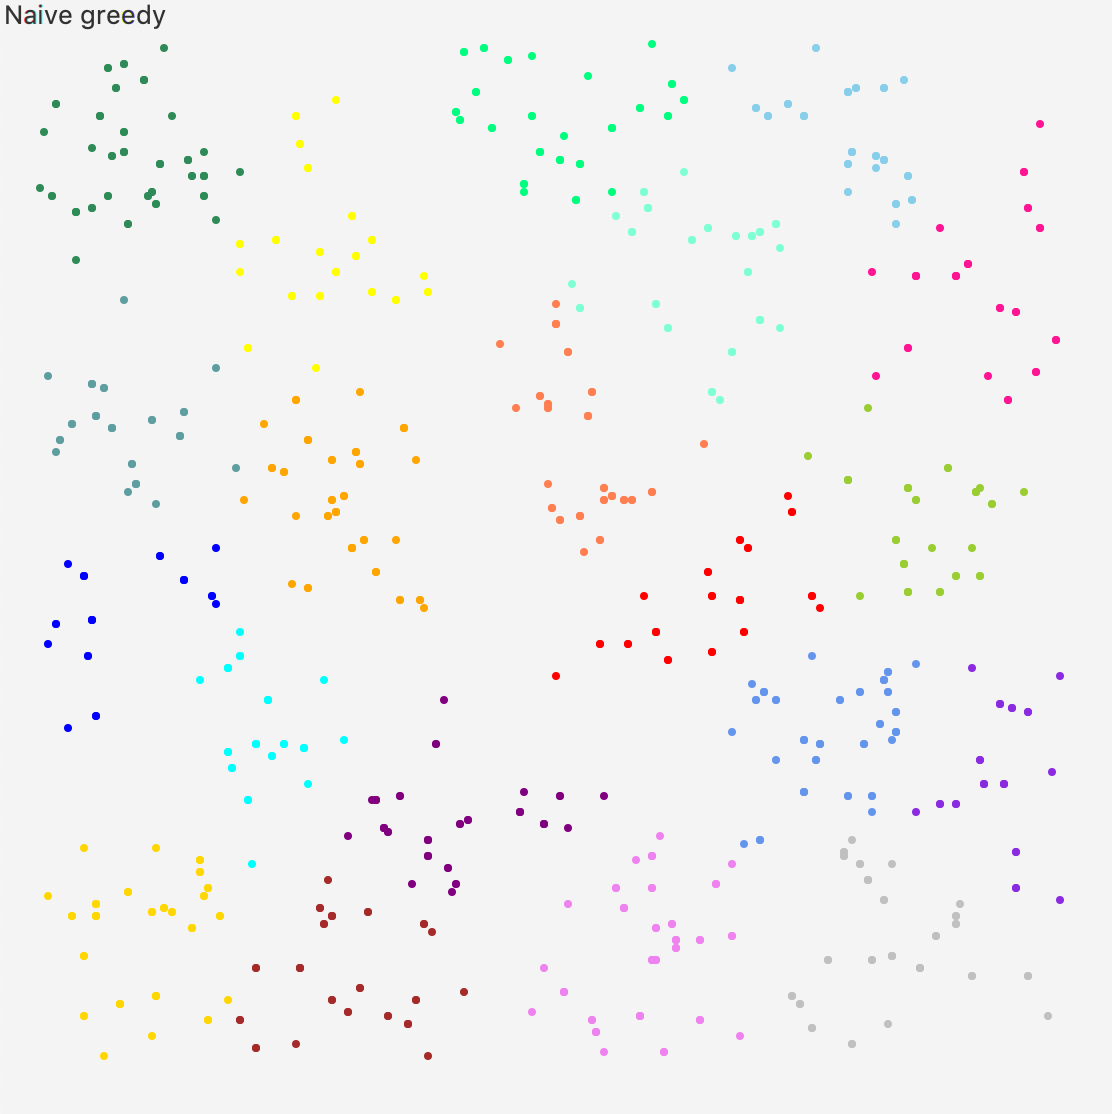
\includegraphics[width=0.45\textwidth]{sprawozdanie_2/naive_greedy.png}
        }
        \subfigure{
           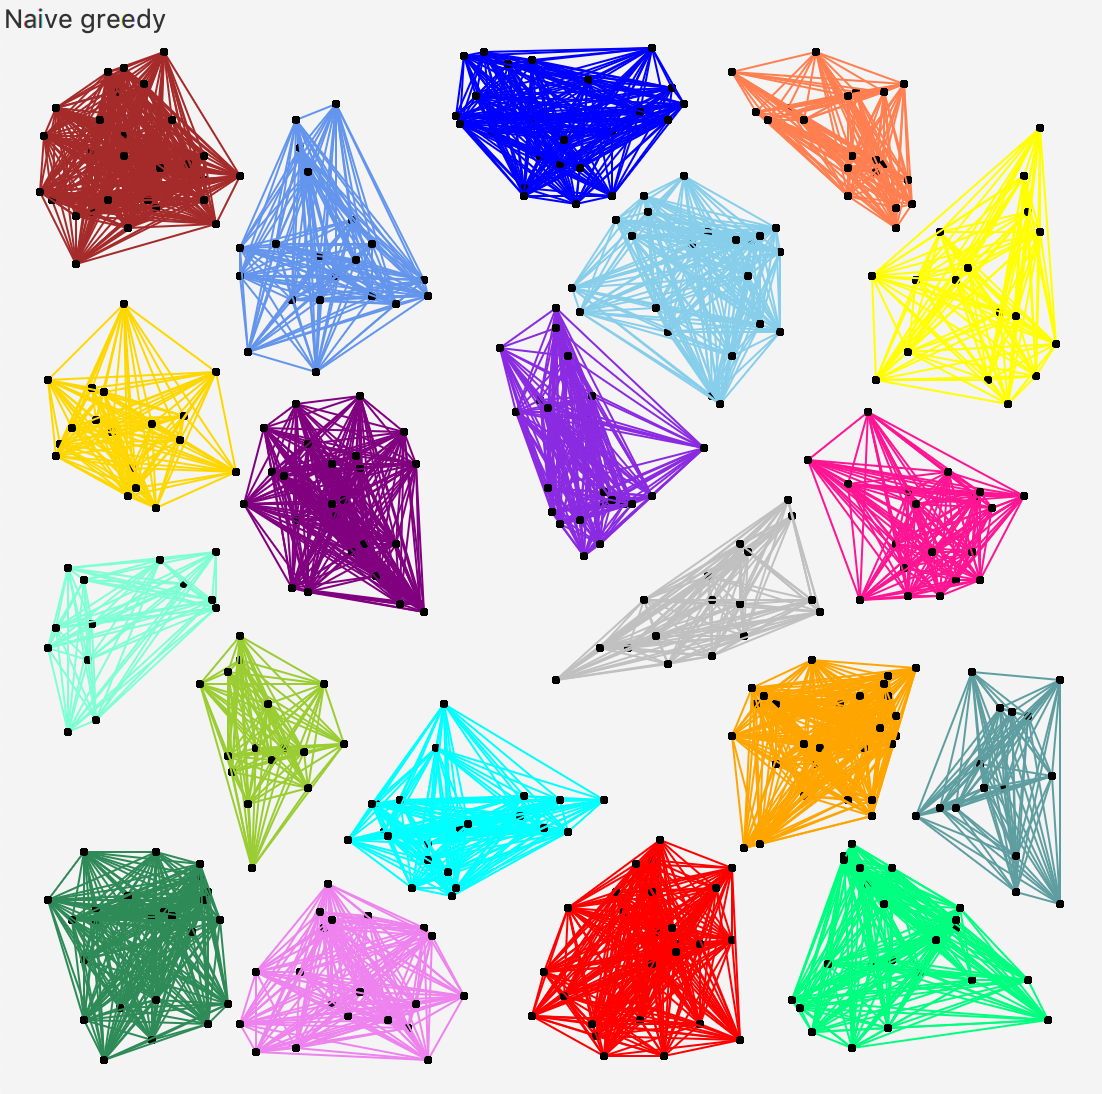
\includegraphics[width=0.45\textwidth]{sprawozdanie_2/naive_greedy_groups.png}
        }\\
        \subfigure{
            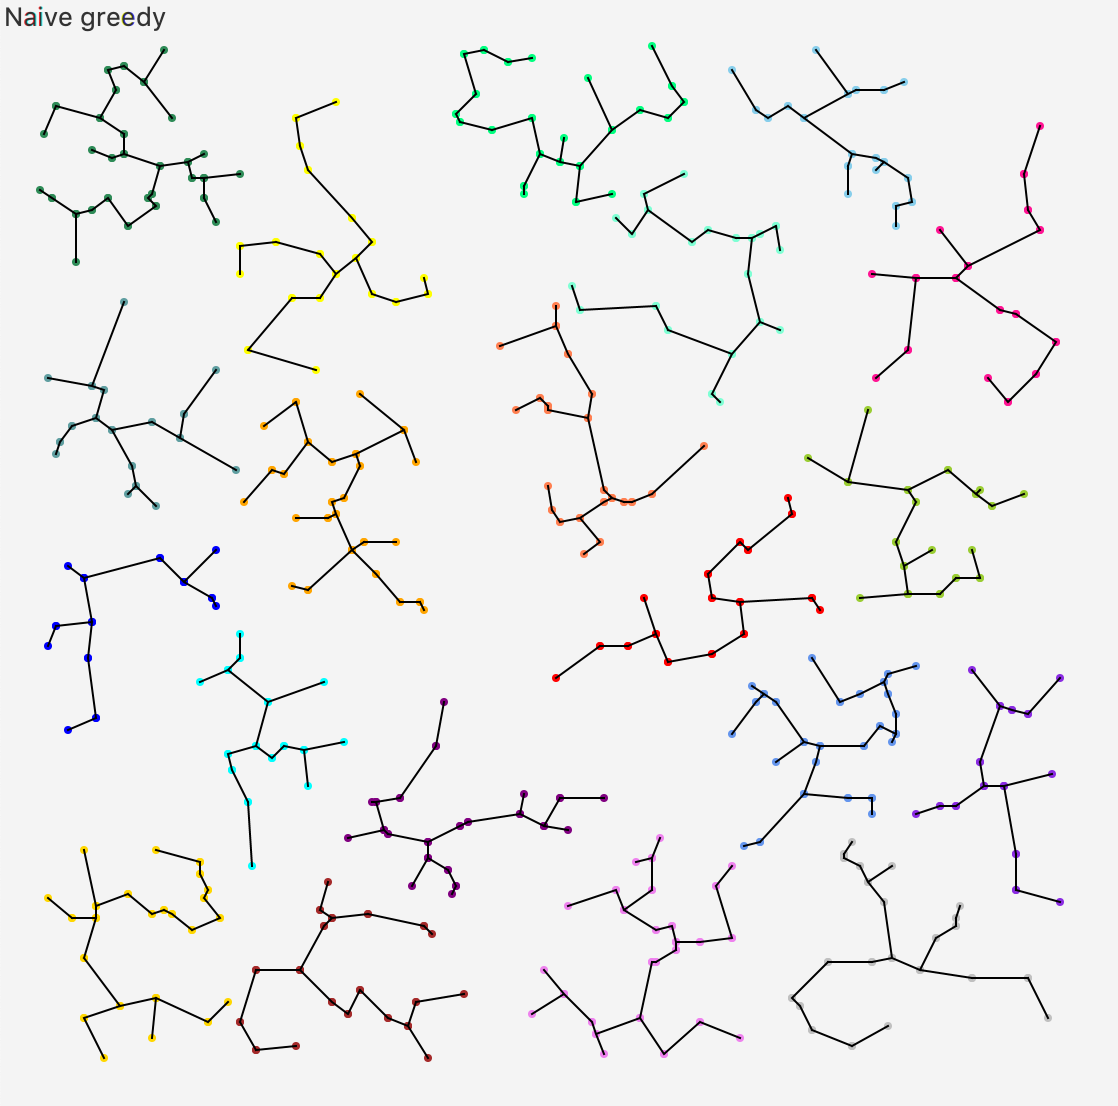
\includegraphics[width=0.45\textwidth]{sprawozdanie_2/naive_greedy_mst.png}
        }
    \end{center}
    \caption{Naive Greedy Local Search}
\end{figure}

\begin{figure}[H]
     \begin{center}
        \subfigure{
            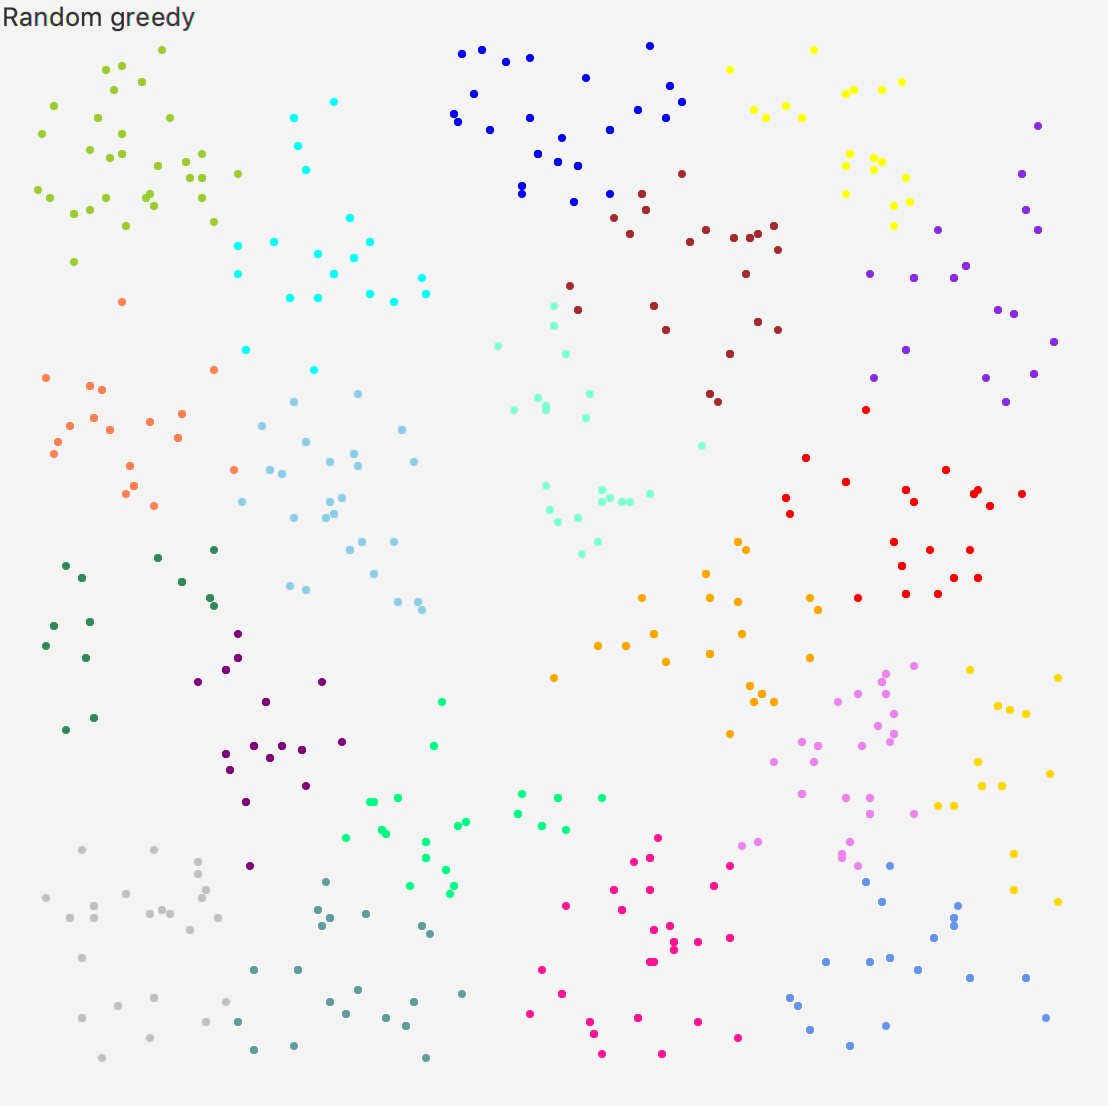
\includegraphics[width=0.45\textwidth]{sprawozdanie_2/random_greedy.png}
        }
        \subfigure{
           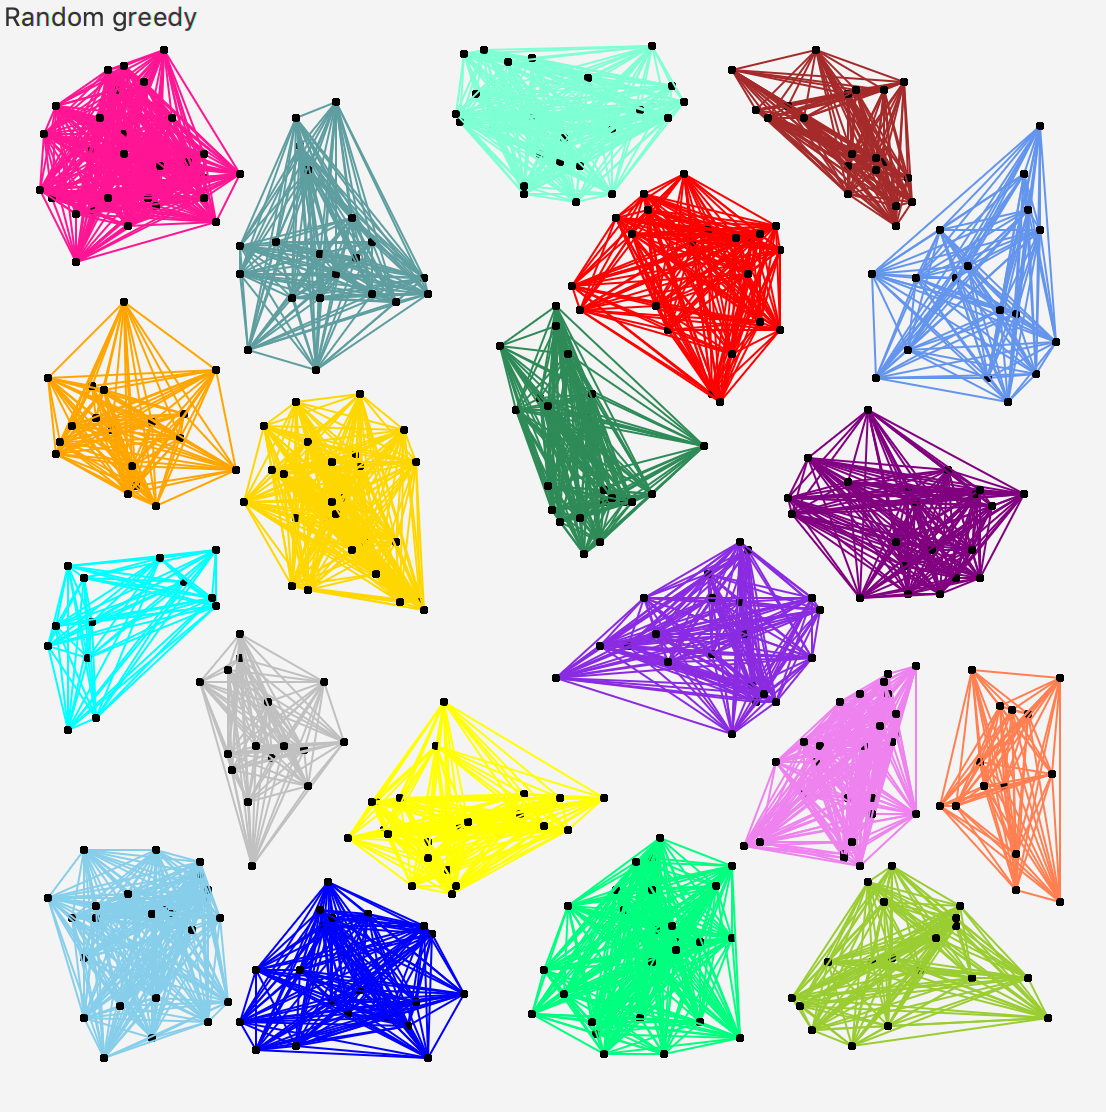
\includegraphics[width=0.45\textwidth]{sprawozdanie_2/random_greedy_groups.png}
        }\\
        \subfigure{
            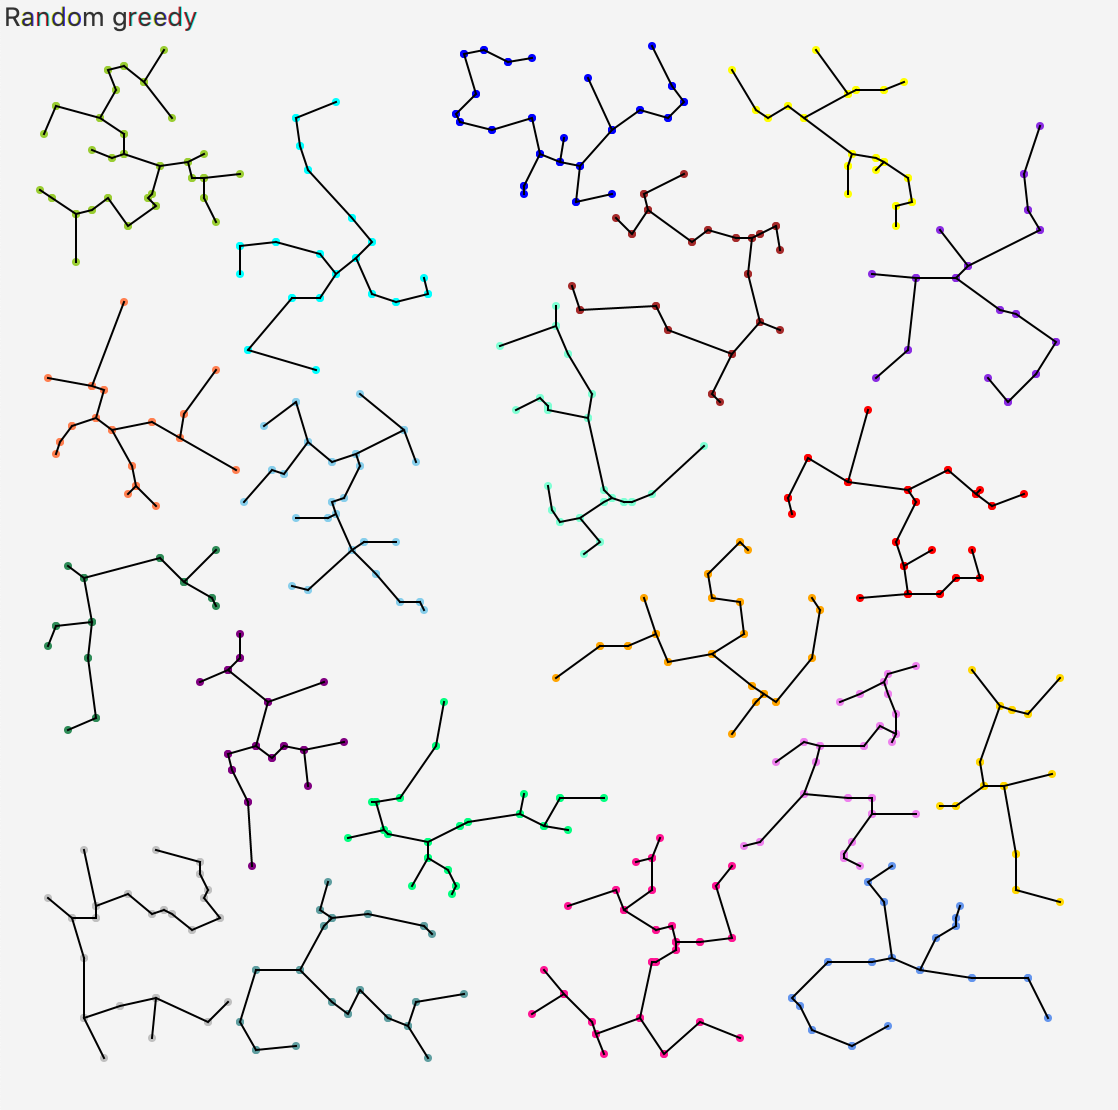
\includegraphics[width=0.45\textwidth]{sprawozdanie_2/random_greedy_mst.png}
        }
    \end{center}
    \caption{Random Greedy Local Search}
\end{figure}

\begin{figure}[H]
     \begin{center}
        \subfigure{
            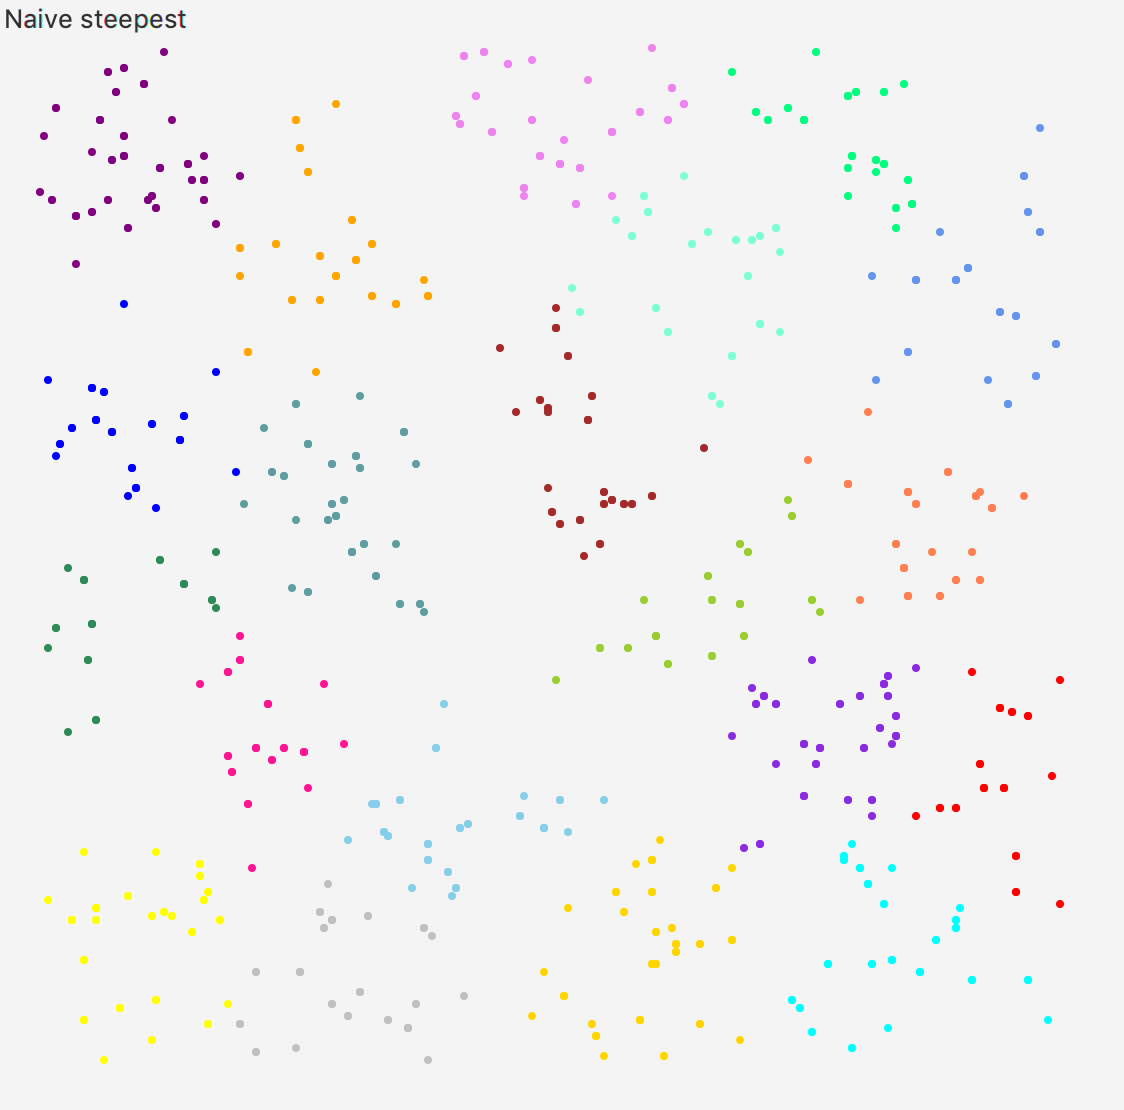
\includegraphics[width=0.45\textwidth]{sprawozdanie_2/naive_steepest.png}
        }
        \subfigure{
           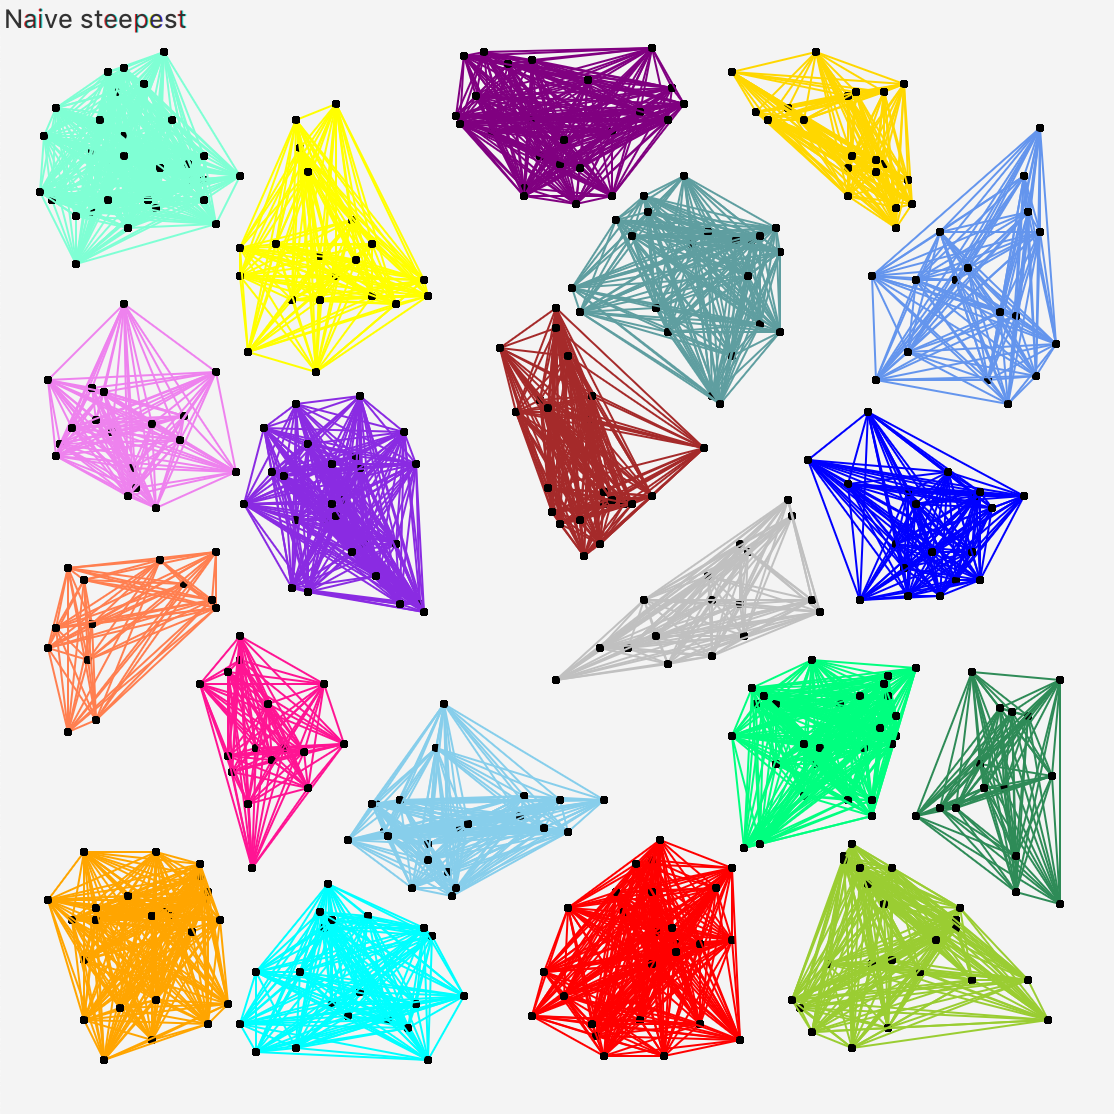
\includegraphics[width=0.45\textwidth]{sprawozdanie_2/naive_steepest_groups.png}
        }\\
        \subfigure{
            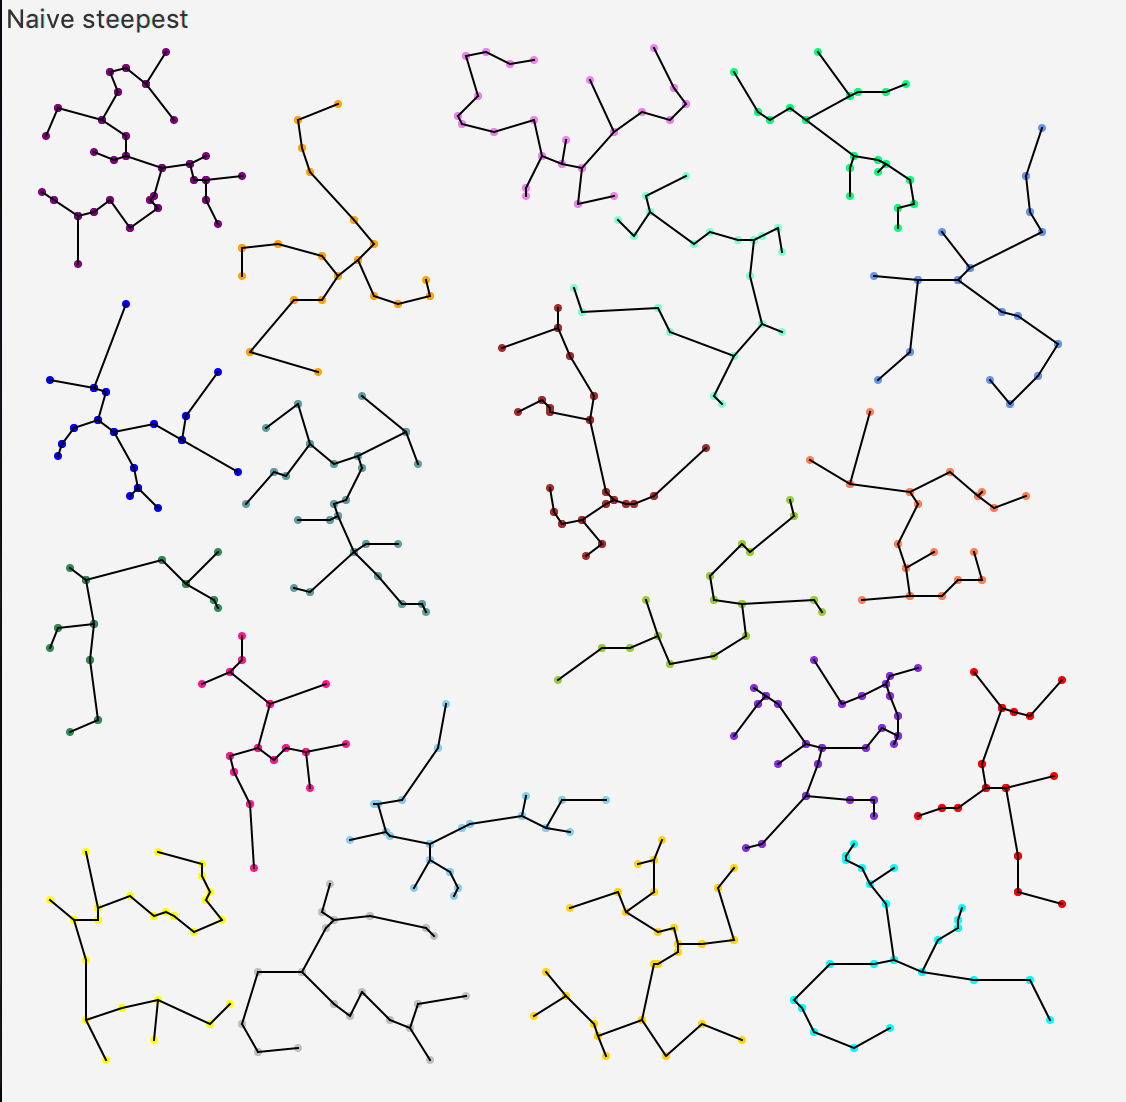
\includegraphics[width=0.45\textwidth]{sprawozdanie_2/naive_steepest_mst.png}
        }
    \end{center}
    \caption{Naive Steepest Local Search}
\end{figure}

\begin{figure}[H]
     \begin{center}
        \subfigure{
            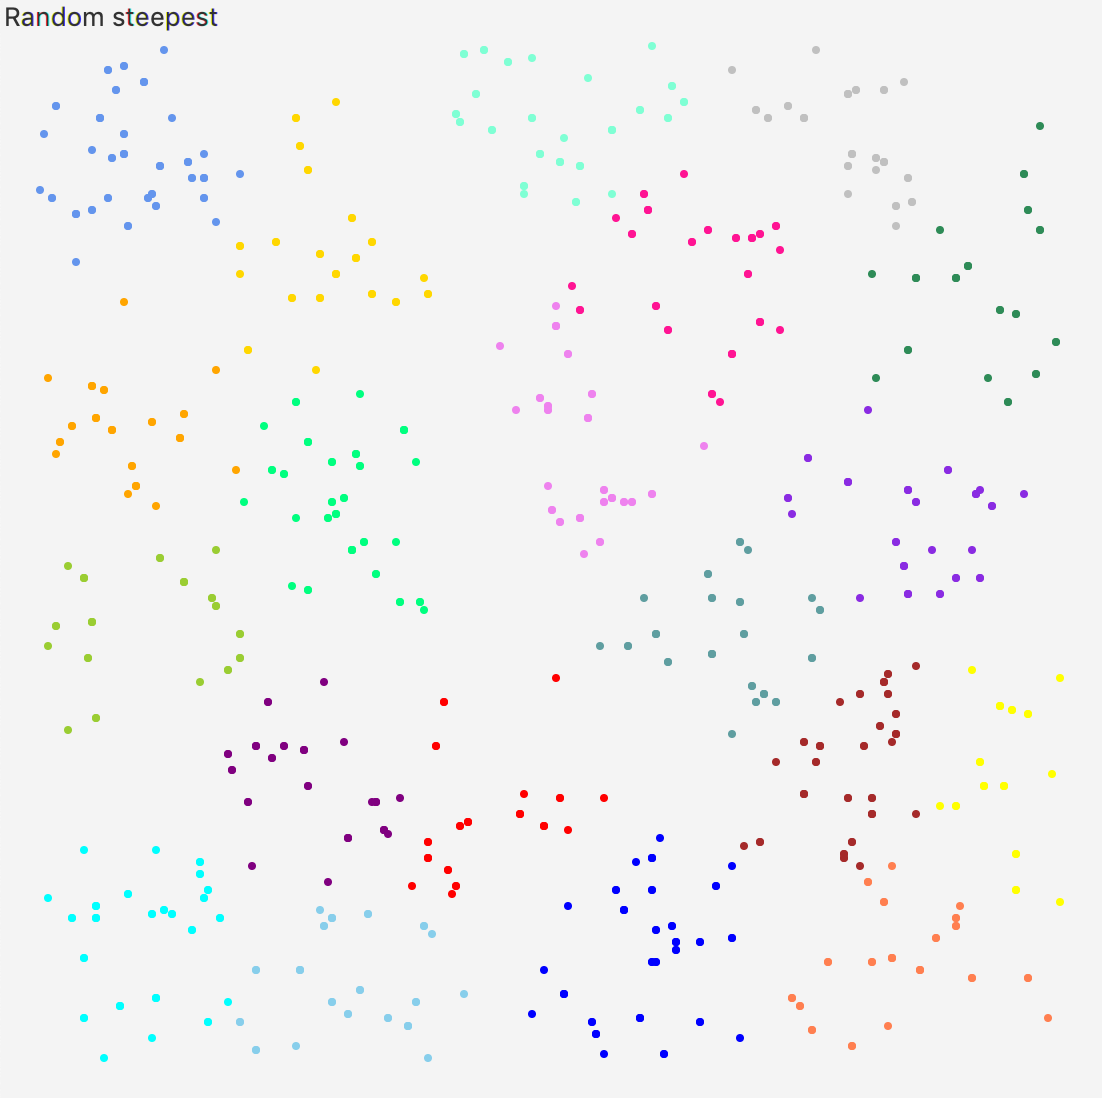
\includegraphics[width=0.45\textwidth]{sprawozdanie_2/random_steepest.png}
        }
        \subfigure{
           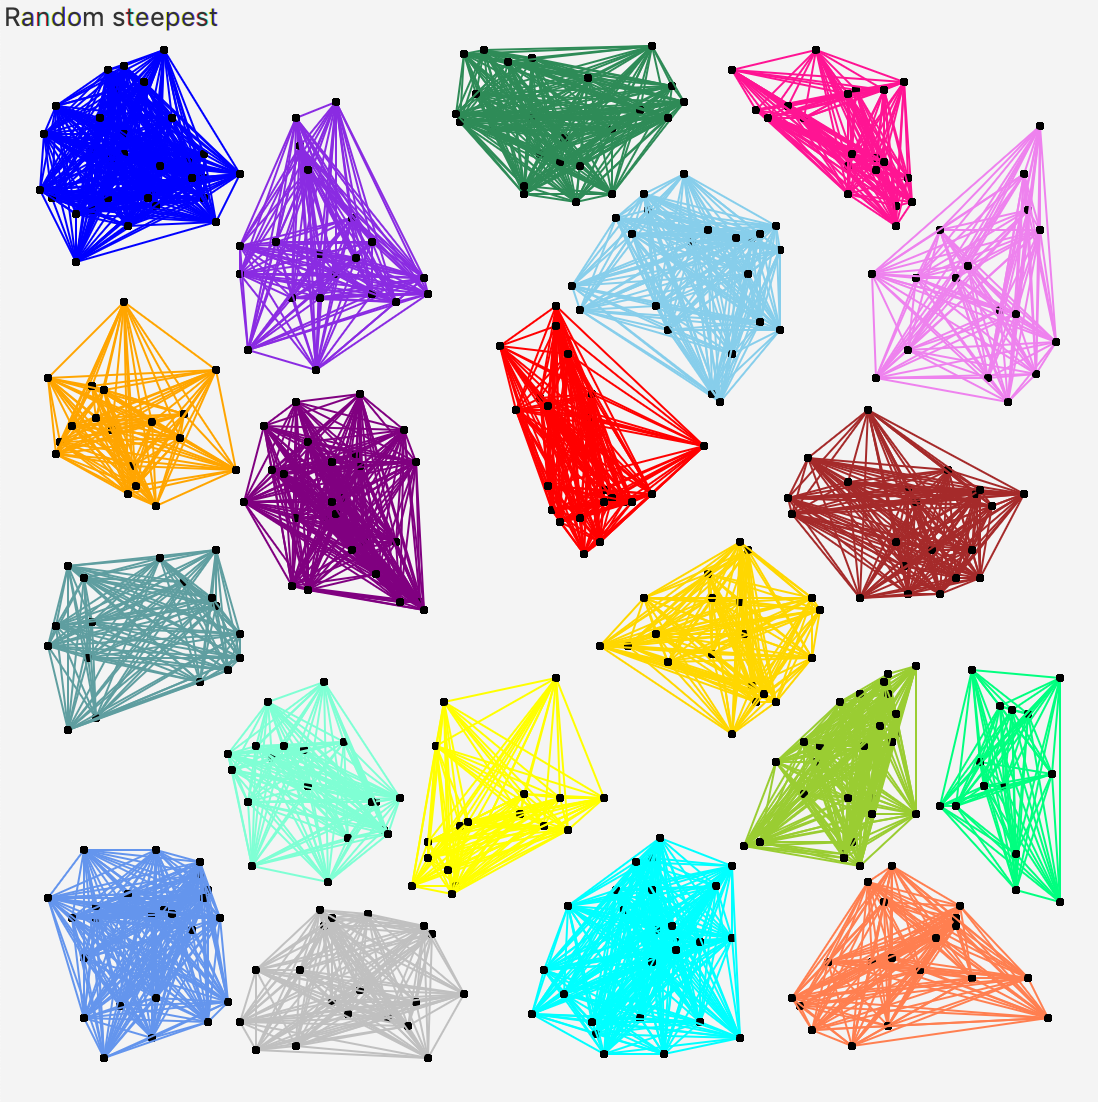
\includegraphics[width=0.45\textwidth]{sprawozdanie_2/random_steepest_groups.png}
        }\\
        \subfigure{
            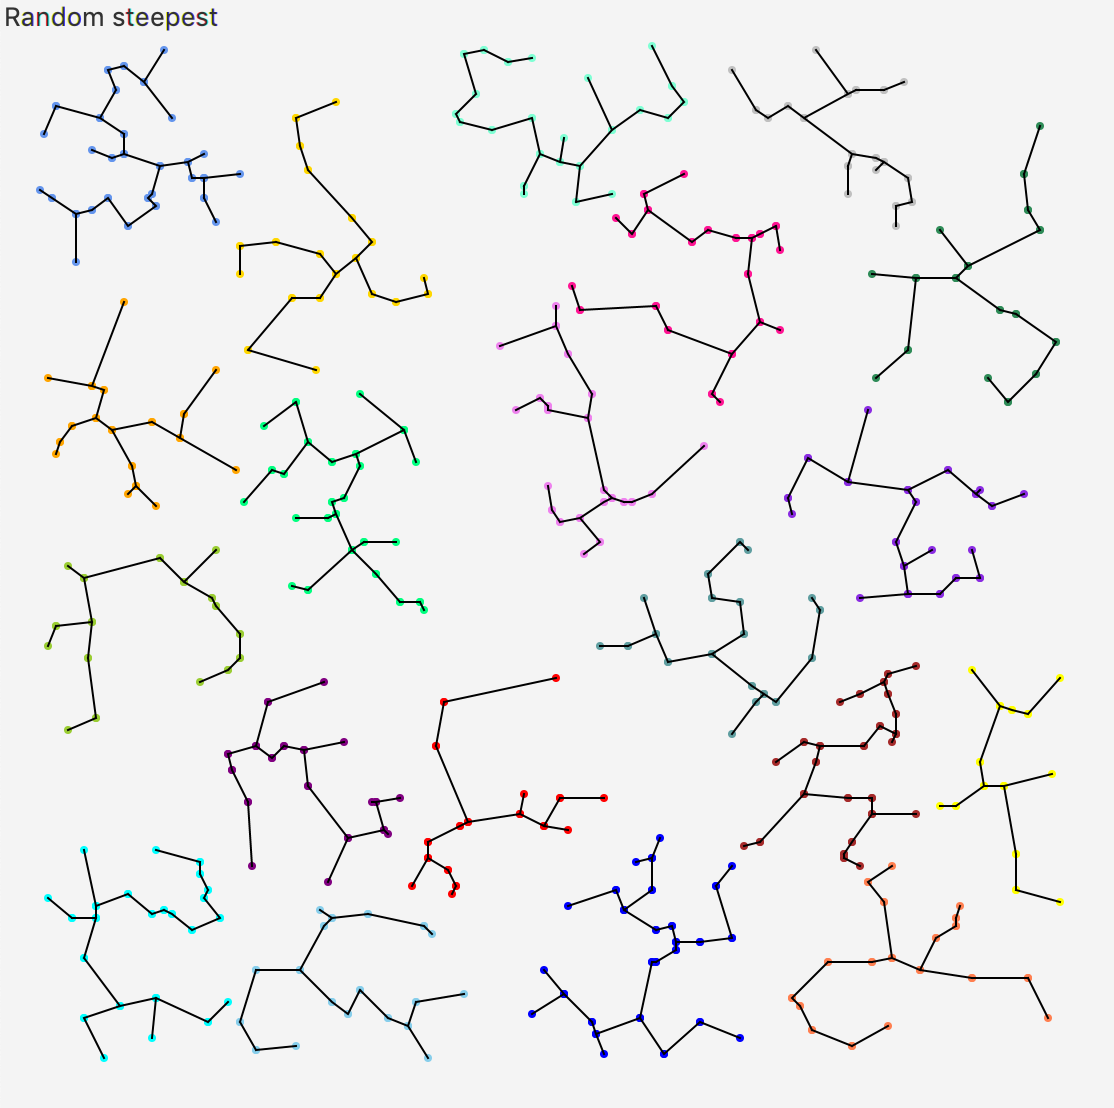
\includegraphics[width=0.45\textwidth]{sprawozdanie_2/random_steepest_mst.png}
        }
    \end{center}
    \caption{Random Steepest Local Search}
\end{figure}

\end{document}